% arara: closeAR
% arara: pdflatex
% arara: pdflatex
% arara: showfile
\documentclass[aspectratio=169]{beamer}

\newcounter{mypage}
\newcounter{mycounter}

\usepackage{tikzlings}
\usetikzlibrary{shapes.callouts}

\colorlet{mycyan}{cyan!30!white} 

\setbeamertemplate{navigation symbols}{}
\setbeamertemplate{background canvas}{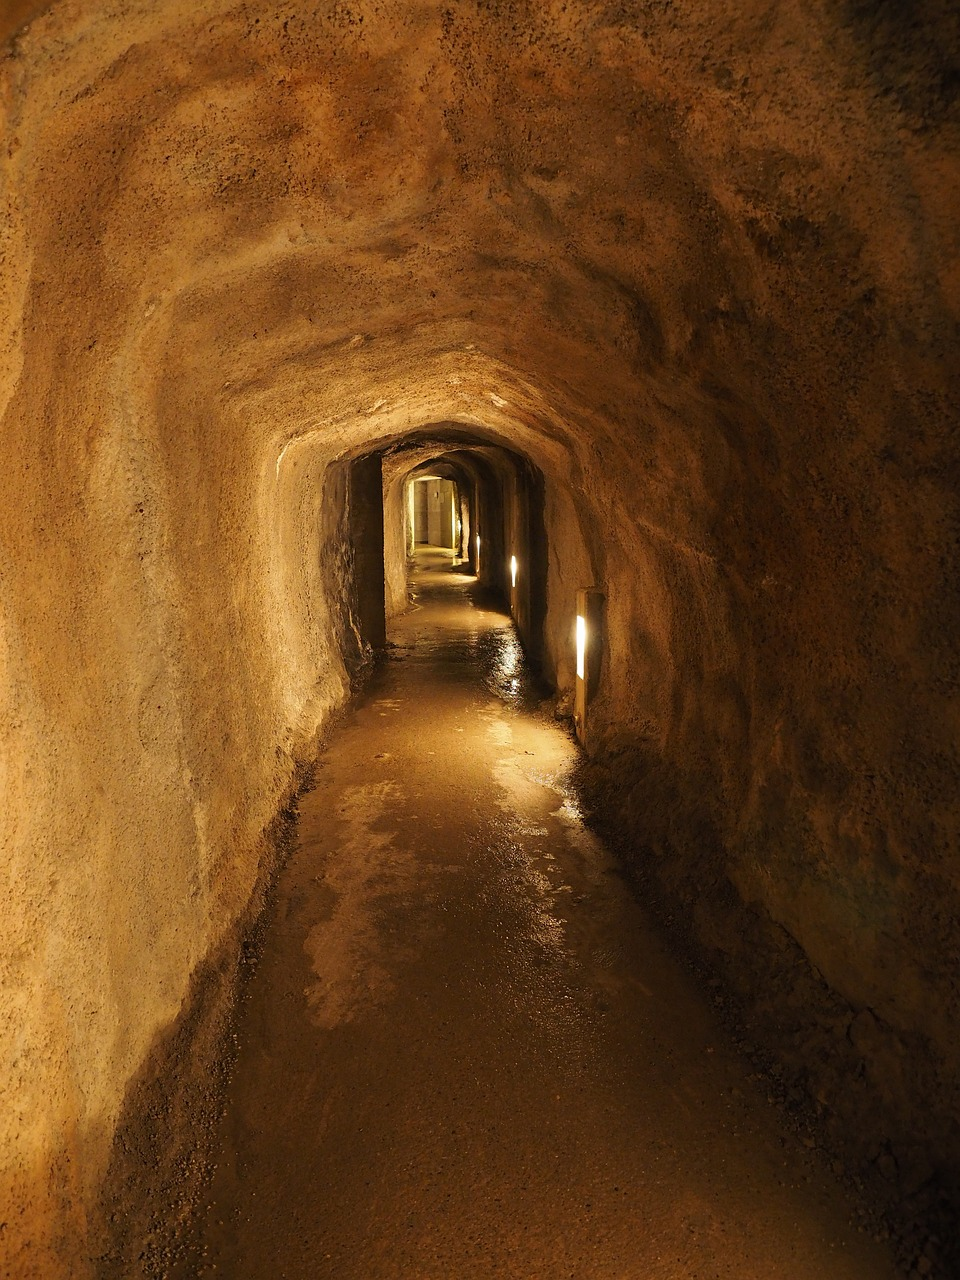
\includegraphics[width=\paperwidth, trim={0 0 0 12cm}, clip]{Back.jpg}}

% trick taken from https://topanswers.xyz/tex?q=1989
\tikzset{
    use page relative coordinates/.style={
        shift={(current page.south west)},
        x={(current page.south east)},
        y={(current page.north west)}
    },
    helmet/.pic={
        \draw[gray, fill=yellow] (-.35,0) -- (-.35,0.2) to[out=90, in=90] (.35,0.2) -- (.35,0) -- cycle;
        \draw[gray, fill=yellow] (-.33,0) to[bend right] (.33,0) -- cycle;
        \draw[gray, fill=white] (0,0.18) circle (1.25mm);
    },
    shovelmole/.pic={
        \moles
    \pic[yshift=1.9cm]
    {helmet};      
    \thing[shovel=black!50!gray,rotate=180, yshift=-2.1cm, xshift=-.5cm]    

     },
    pickaxemole/.pic={
        \moles
        \pic[yshift=1.9cm]
    {helmet};
    \thing[pickaxe=black!50!gray,rotate=180, yshift=-2.1cm, xshift=-.5cm]
    },
  }

\begin{document}
\begin{frame}
  \begin{tikzpicture}[remember picture, overlay,use page relative coordinates]
     % credit for background image
    \node[white,text width=.7\paperwidth,font=\tiny,align=center] at ([yshift=0.35cm]current page.south) {Image source: \href{https://pixabay.com/de/photos/stollen-gang-unterirdisch-säntis-505977/}{https://pixabay.com/de/photos/stollen-gang-unterirdisch-säntis-505977/}};
  \end{tikzpicture}
  \begin{tikzpicture}[remember picture, overlay, xshift=6.3cm]
    \pic[scale=.3+\thepage/150, xshift=-2cm, yshift=-3.72cm-.08\thepage cm, transform shape] {shovelmole};
    \pic[scale=.3+\thepage/150, yshift=-3.72cm-.08\thepage cm, transform shape] {pickaxemole};
    \pic[scale=.3+\thepage/150, xshift=2cm, yshift=-3.72cm-.08\thepage cm, transform shape] {shovelmole};
  \end{tikzpicture}
 \pause[110]
 \setcounter{mypage}{\value{page}}
\end{frame}	
 \begin{frame}
   \begin{tikzpicture}[remember picture, overlay,use page relative coordinates]
     % credit for background image
     \node[white,text width=.7\paperwidth,font=\tiny,align=center] at ([yshift=0.35cm]current page.south) {Image source: \href{https://pixabay.com/de/photos/stollen-gang-unterirdisch-säntis-505977/}{https://pixabay.com/de/photos/stollen-gang-unterirdisch-säntis-505977/}};    
   \end{tikzpicture}\stepcounter{mycounter}
   \begin{tikzpicture}[remember picture, overlay, xshift=6.3cm]
     \pic[scale=.3+\themypage/150, xshift=-2cm,  yshift=-3.72cm-.08\themypage cm, transform shape] {shovelmole};
     \pic[scale=.3+\themypage/150,  yshift=-3.72cm-.08\themypage cm, transform shape] {pickaxemole};
     \pic[scale=.3+\themypage/150, xshift=2cm,  yshift=-3.72cm-.08\themypage cm, transform shape] {shovelmole};
    \ifnumgreater{\themycounter}{0}{%
      \draw[fill=mycyan] (-2.2,-1.4) ellipse[x radius=.1cm,y radius=.05cm];
      \draw[fill=mycyan] (0,-1.4) ellipse[x radius=.1cm,y radius=.05cm];
      \draw[fill=mycyan] (2.2,-1.4) ellipse[x radius=.1cm,y radius=.05cm];
    }{}
    \ifnumgreater{\themycounter}{1}{%
      \draw[fill=mycyan] (-2.4,-1.2) ellipse[x radius=.15cm,y radius=.1cm];
      \draw[fill=mycyan] (0,-1.2) ellipse[x radius=.15cm,y radius=.1cm];
      \draw[fill=mycyan] (2.4,-1.2) ellipse[x radius=.15cm,y radius=.1cm];
    }{}
    \ifnumgreater{\themycounter}{2}{%
      \draw[fill=mycyan] (-2.6,-.9) ellipse[x radius=.2cm,y radius=.15cm];
      \draw[fill=mycyan] (0,-.9) ellipse[x radius=.2cm,y radius=.15cm];
      \draw[fill=mycyan] (2.6,-.9) ellipse[x radius=.2cm,y radius=.15cm];
    }{}
    \ifnumgreater{\themycounter}{3}{%
      \node[cloud, draw, fill=mycyan, aspect=1.5, text width=1.2cm, yshift=.08cm, xshift=-3cm] {};
      \node[cloud, draw, fill=mycyan, aspect=1.5, text width=1.2cm, yshift=.2cm] {};
      \node[cloud, draw, fill=mycyan, aspect=1.5, text width=1.2cm, yshift=.08cm, xshift=3cm] {};
    }{}    
%    \ifnumgreater{\themycounter}{4}{%
%      \chicken[body=brown, scale=.4, yshift=-.88cm, xshift=-7.5cm]
%      \bat[scale=.4, yshift=-.7cm]
%      \owl[scale=.4, yshift=-.88cm, xshift=7.5cm]
%    }{}    
   \ifnumgreater{\themycounter}{4}{%
     \owl[scale=.4, yshift=-.88cm, xshift=-7.5cm]
     \bee[wings=white, scale=.4, yshift=-.7cm]
     \chicken[body=brown, scale=.4, yshift=-.88cm, xshift=7.5cm]
    }{}    
  \end{tikzpicture}
  \pause[5]
\end{frame}	
\end{document}